\documentclass{standalone}
\usepackage{tikz}
\begin{document}
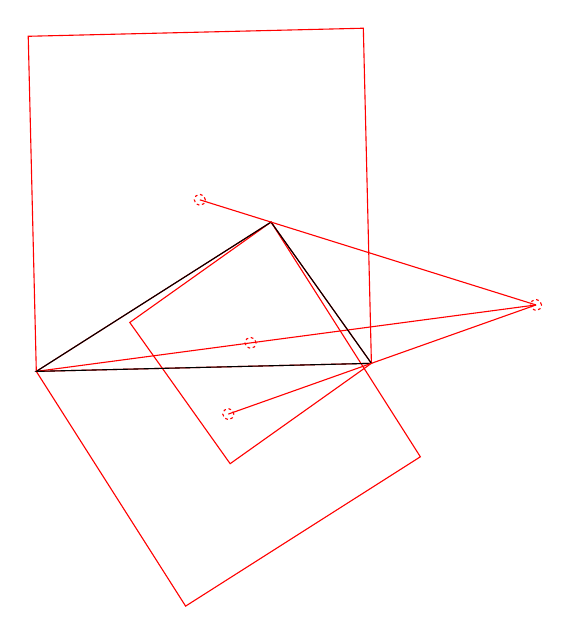
\begin{tikzpicture}[x=1pt,y=1pt]
\draw[red] (89.70,-156.91) -- (210.79,-154.00) -- (207.87,-32.91) -- (86.78,-35.82) -- cycle;
\draw[red] (174.52,-102.95) -- (89.70,-156.91) -- (143.65,-241.73) -- (228.47,-187.77) -- cycle;
\draw[red] (270.26,-132.90) -- (89.70,-156.91);
\draw[red, dash pattern=on 1pt] (148.79,-94.91) circle (2.00);
\draw[red, dash pattern=on 1pt] (167.13,-146.61) circle (2.00);
\draw[red, dash pattern=on 1pt] (159.08,-172.34) circle (2.00);
\draw[red, dash pattern=on 1pt] (270.26,-132.90) circle (2.00);
\draw[red] (210.79,-154.00) -- (174.52,-102.96) -- (123.47,-139.23) -- (159.74,-190.26) -- cycle;
\draw (89.70,-156.91) -- (210.79,-154.00) -- (174.52,-102.96) -- cycle;
\draw[red] (270.26,-132.90) -- (159.08,-172.34);
\draw[red] (270.26,-132.90) -- (148.79,-94.91);
\end{tikzpicture}
\end{document}
